\documentclass{standalone}

\usepackage[T1]{fontenc}
\usepackage[utf8]{inputenc}
\usepackage{eulervm}
\usepackage{amsmath}
\usepackage{bm}
\usepackage{tikz}
\usepackage{environ}

\usetikzlibrary{fit}
\usetikzlibrary{patterns}
\usetikzlibrary{arrows}

\input{colors}

\begin{document}
  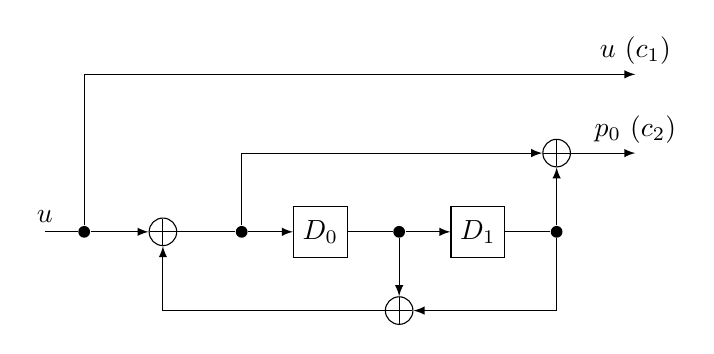
\begin{tikzpicture}%[scale=\tikzscale]

  \tikzset{XOR/.style={draw,circle, minimum height=0.35cm,append after command={
          [shorten >=\pgflinewidth, shorten <=\pgflinewidth,]
          (\tikzlastnode.north) edge (\tikzlastnode.south)
          (\tikzlastnode.east) edge (\tikzlastnode.west)
          }
      }
  }

  \tikzset{STA/.style={draw, minimum height=0.65cm, minimum width=0.65cm} }

  \node (d0) at (0.0,0.0) [circle,fill,inner sep=1.5pt]{};
  \node (d1) at (2.0,0.0) [circle,fill,inner sep=1.5pt]{};
  \node (d2) at (4.0,0.0) [circle,fill,inner sep=1.5pt]{};
  \node (d3) at (6.0,0.0) [circle,fill,inner sep=1.5pt]{};

  \node[STA] (s0) at (3.0, 0.0) {$D_0$};
  \node[STA] (s1) at (5.0, 0.0) {$D_1$};

  \node[XOR] (x0) at (1.0,  0.0) {};
  \node[XOR] (x1) at (4.0, -1.0) {};
  \node[XOR] (x2) at (6.0,  1.0) {};

  \draw[->,>=latex] (d0) -- (x0);
  \draw[- ,>=latex] (x0) -- (d1);
  \draw[->,>=latex] (d1) -- (s0);
  \draw[- ,>=latex] (s0) -- (d2);
  \draw[->,>=latex] (d2) -- (x1);
  \draw[->,>=latex] (d2) -- (s1);
  \draw[- ,>=latex] (s1) -- (d3);
  \draw[->,>=latex] (d3) |- (x1);
  \draw[->,>=latex] (x1) -| (x0);
  \draw[->,>=latex] (d1) |- (x2);
  \draw[->,>=latex] (d3) -- (x2);

  \draw[->,>=latex] (x2) -- (7.0, 1.0) node [right, above] {$p_0~(c_2)$};
  \draw[->,>=latex] (d0) |- (7.0, 2.0) node [right, above] {$u~(c_1)$};
  \draw[- ,>=latex] (-0.5,0.0) node [left,  above] {$u$} -- (d0);
  \end{tikzpicture}
\end{document}